%%%%%%%%%%%%%%%%%%%%%%%%
%
% $Autor: Sadegh Naderi $
% $Datum: 2023-11-24  $
% $Short Description: Description of the TensorFlow package $
% $Directory: ML23-01-Keyword-Spotting-with-an-Arduino-Nano-33-BLE-Sense\report\Contents\en\TensorFlow.tex $
% $Version: 7.0 $
%
%%%%%%%%%%%%%%%%%%%%%%%%


\chapter{TensorFlow}


\section{Introduction}

In the ever-evolving landscape of machine learning and artificial intelligence, TensorFlow stands as a cornerstone library, empowering developers and researchers with a robust platform for numerical computations. Originally developed by the Google Brain team, TensorFlow has become a driving force behind large-scale services at Google, including Google Cloud Speech, Google Photos, and Google Search. Since its open-source debut in November 2015, TensorFlow has grown to be the most widely adopted deep learning library in the industry.

TensorFlow's appeal lies in its ability to seamlessly blend flexibility and efficiency, offering a versatile toolkit for a myriad of machine learning applications. From image classification and natural language processing to recommender systems and time series forecasting, TensorFlow provides a comprehensive framework that scales from research experiments to real-world applications.

It enables the training and execution of very large neural networks efficiently by distributing computations across potentially hundreds of multi-GPU servers \cite{Geron:2022}:

\begin{itemize}
	\item \textbf{Origin:} TensorFlow was created at Google and supports many of its large-scale machine learning applications.
	
	\item \textbf{Open Source:} TensorFlow was open-sourced in November 2015.
	
	\item \textbf{Version:} Version 2.0 was released in September 2019.
	
	\item \textbf{Integration with Keras:} TensorFlow comes bundled with Keras, and Keras relies on TensorFlow for all intensive computations.
\end{itemize}

\subsection{TensorFlow Framework}

\subsubsection{TensorFlow Overview}

TensorFlow serves as a scalable machine learning system operating in diverse environments. Employing dataflow graphs to represent computation, shared state, and state-altering operations, TensorFlow is proficient in training and executing deep neural networks for various applications, including handwritten digit classification, image recognition, word embeddings, recurrent neural networks, sequence-to-sequence models for machine translation, natural language processing, and PDE-based simulations. The framework efficiently maps dataflow graph nodes across multiple machines in a cluster and across various computational devices within a machine, such as multicore CPUs, general-purpose GPUs, and specialized ASICs known as Tensor Processing Units (TPUs). TensorFlow facilitates experimentation with novel optimizations and training algorithms, with a primary focus on deep neural network training and inference. Widely used in Google services, TensorFlow is released as an open-source project and has become a staple in machine learning research, showcasing compelling performance across real-world applications.

\subsubsection{TensorFlow Use Case}

TensorFlow, developed by Google, is a versatile framework for creating machine learning applications and training models. Google's search engine itself relies on TensorFlow for AI applications. For instance, when a user types a query into the Google search bar, the search engine predicts the most suitable word completion based on previous searches. TensorFlow is applicable across various tasks, with a particular emphasis on training and inferring deep neural networks. It offers diverse workflows for model development and training using programming languages like Python and JavaScript. After training, models can be deployed on the cloud or any device for edge computing applications, regardless of the language used on the device. The crucial aspect of every machine learning application is training the model to make real-time decisions without human intervention.

\subsubsection{TensorFlow Lite for Microcontrollers}

TensorFlow is a crucial piece of infrastructure for training machine learning models and teaching algorithms to identify patterns in data. However, when deploying on small embedded microcontrollers, the need arises to streamline TensorFlow for efficiency. TensorFlow Lite, or TFLite, addresses this need by providing tools to convert and optimize TensorFlow models for mobile and edge devices. It is designed to be lean and mean, catering to the requirements of resource-constrained edge devices. TensorFlow Lite for Microcontrollers is specifically tailored for running on devices with limited memory, enabling the enhancement of intelligence in billions of devices, including household appliances and Internet of Things (IoT) devices. This implementation brings machine learning to tiny microcontrollers, reducing dependence on expensive hardware or reliable internet connections and ensuring data security by keeping data on the device. TensorFlow Lite excels in on-device machine learning (Edge ML) and is optimized for deployment to resource-constrained edge devices \cite{Dokic:2020}.



\section{Description}

\subsection{Overview of TensorFlow}

TensorFlow stands out as a potent library for numerical computations \cite{Geron:2022}, especially tailored for extensive machine learning applications (though it can be employed for any task demanding substantial computations). Developed by the Google Brain team, TensorFlow drives various large-scale services at Google, including Google Cloud Speech, Google Photos, and Google Search. Open-sourced in November 2015, it has since become the most widely utilized deep learning library in the industry. Countless projects leverage TensorFlow for diverse machine learning tasks, such as image classification, natural language processing, recommender systems, and time series forecasting.

So, what does TensorFlow provide? Here is a summary:

\begin{itemize}
	\item Its core closely resembles NumPy but with GPU support.
	\item It supports distributed computing across multiple devices and servers.
	\item It incorporates a just-in-time (JIT) compiler optimizing computations for speed and memory usage by extracting and optimizing the computation graph.
	\item Computation graphs can be exported to a portable format, allowing training in one environment and running in another.
	\item It implements reverse-mode autodiff and offers excellent optimizers like RMSProp and Nadam.
\end{itemize}

TensorFlow offers numerous features built upon these core capabilities, with Keras being the most notable. Additionally, it includes data loading and preprocessing operations (tf.data, tf.io, etc.), image processing operations (tf.image), signal processing operations (tf.signal), and more.

At the lowest level, each TensorFlow operation (op) is implemented using highly efficient C++ code, with multiple implementations called kernels dedicated to specific device types like CPUs, GPUs, or TPUs (tensor processing units). GPUs and TPUs significantly accelerate computations.

\begin{figure}[h!]
	\centering
	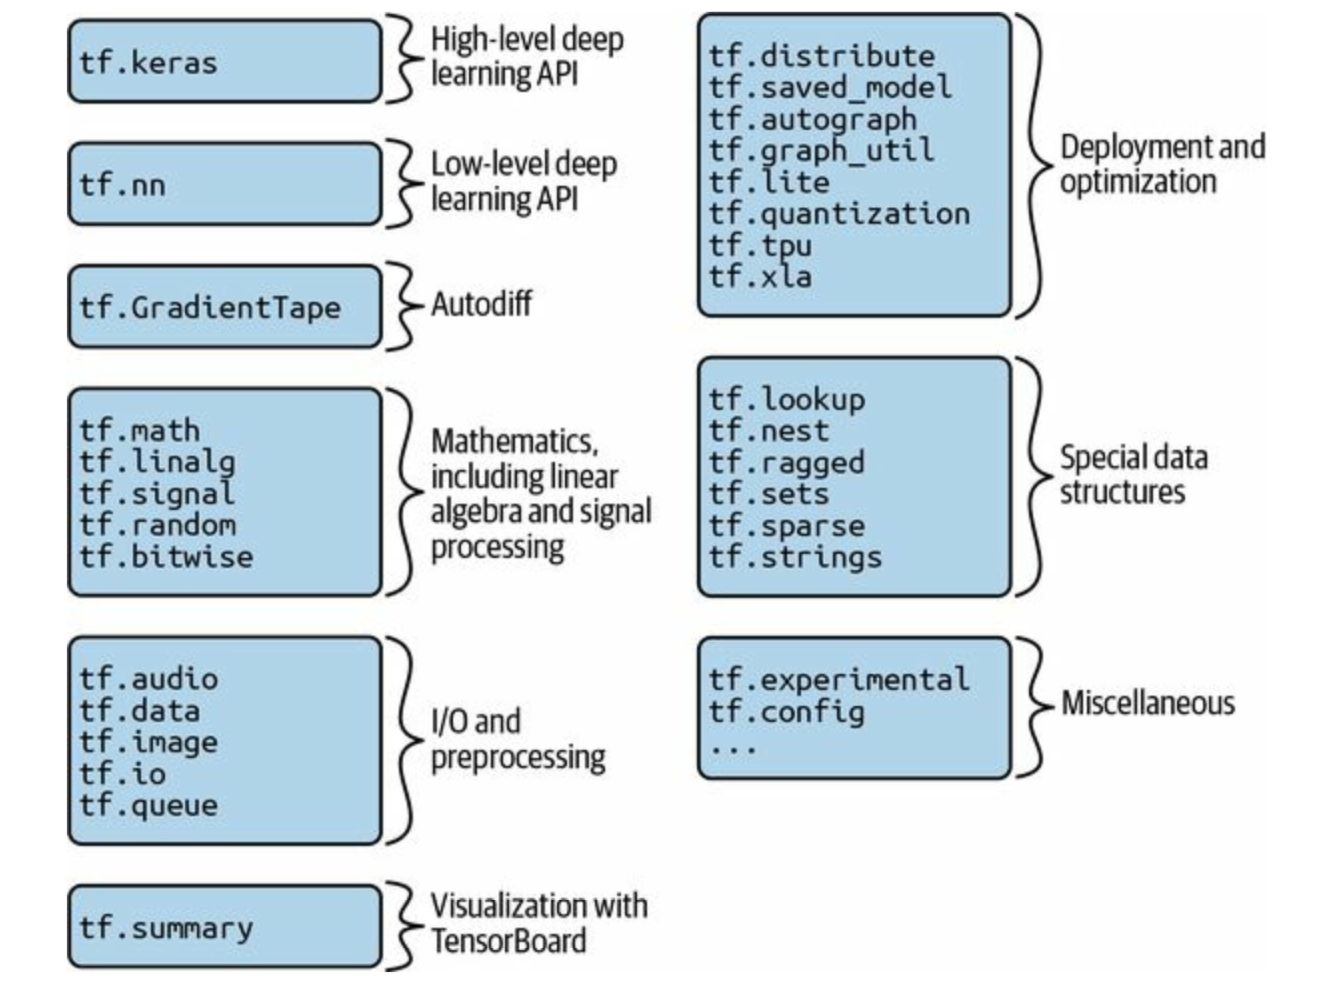
\includegraphics[width=0.9\textwidth]{Images/TensorFlow/tensorflowPythonAPI}
	\caption{TensorFlow’s Python API \cite{Geron:2022}} 
	\label{fig:tensorflowAPI}
\end{figure}



TensorFlow's architecture, depicted in Figure~\ref{fig:tensorflowAPI}, illustrates that while high-level APIs like Keras and tf.data are often used, the lower-level Python API allows direct handling of tensors. TensorFlow's execution engine efficiently manages operations, even across multiple devices and machines if specified.

TensorFlow runs on Windows, Linux, macOS, and mobile devices through TensorFlow Lite, supporting both iOS and Android. APIs for other languages, including C++, Java, Swift, and TensorFlow.js (JavaScript implementation), are also available.

\begin{figure}[h!]
	\centering
	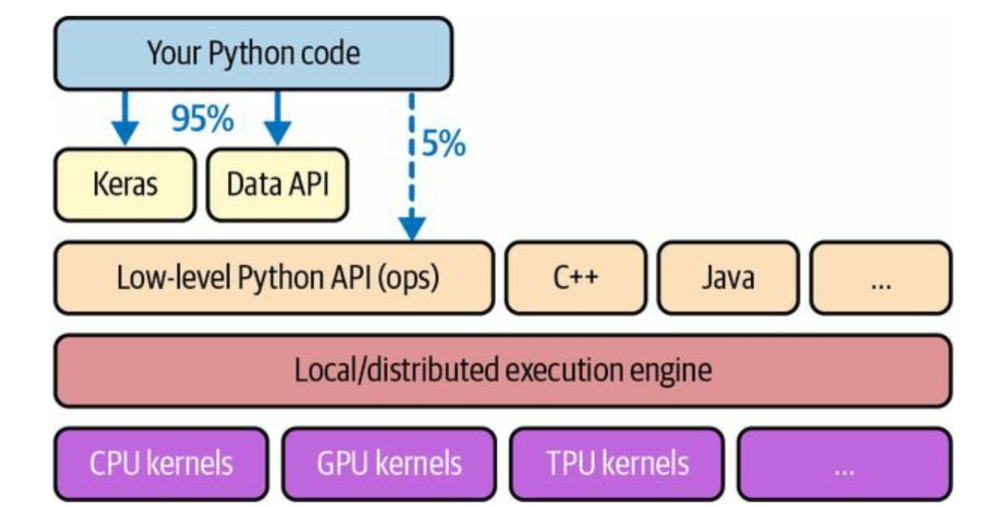
\includegraphics[width=0.8\textwidth]{Images/TensorFlow/tensorflowArchitecture}
	\caption{TensorFlow’s architecture \cite{Geron:2022}}
	\label{fig:tensorflowArchitecture}
\end{figure}


Beyond being a library, TensorFlow anchors an extensive ecosystem of libraries. TensorBoard aids visualization, and TensorFlow Extended (TFX) by Google helps in the productionization of TensorFlow projects, offering tools for data validation, preprocessing, model analysis, and serving. TensorFlow Hub facilitates easy downloading and reuse of pretrained neural networks. The TensorFlow model garden provides various neural network architectures, some pretrained. Explore TensorFlow Resources, \texttt{https://github.com/jtoy/awesome-tensorflow}, for more TensorFlow-based projects, and find numerous projects on GitHub.

\subsection{Data Structures Supported}

TensorFlow supports many data structures \cite{Geron:2022}:

\begin{itemize}
	\item \textbf{Tensors (\PYTHON{tf.Tensor}):} The essence of TensorFlow's API centers on tensors, which traverse from one operation to another, hence the name TensorFlow. A tensor closely resembles a NumPy ndarray, typically representing a multidimensional array but capable of containing a scalar, like a simple value such as 42. The significance of these tensors becomes evident as we delve into creating custom cost functions, metrics, layers, and additional functionalities.
	
	\item \textbf{Variables (\PYTHON{tf.Variable}):} A tf.Variable behaves akin to a tf.Tensor: you can carry out similar operations, seamlessly integrate it with NumPy, and it exhibits the same strictness with types. However, it distinguishes itself by being mutable, allowing modifications in place.
	
 	\item \textbf{Sparse Tensors (\PYTHON{tf.SparseTensor}):}
	Efficiently represent tensors containing mostly zeros. The tf.sparse package contains operations for sparse tensors.
	
	\item \textbf{Tensor Arrays (\PYTHON{tf.TensorArray}):}
	Lists of tensors with a default fixed length, but can optionally be made extensible. All tensors they contain must have the same shape and data type.
	
	\item \textbf{Ragged Tensors (\PYTHON{tf.RaggedTensor}):}
	Represent lists of tensors with the same rank and data type, but varying sizes. The dimensions along which the tensor sizes vary are called the ragged dimensions. The tf.ragged package contains operations for ragged tensors.
	
	\item \textbf{String Tensors:}
	Regular tensors of type \PYTHON{tf.string} representing byte strings, not Unicode strings. Unicode strings can be represented using tensors of type tf.int32. The tf.strings package contains ops for byte strings and Unicode strings.
	
	\item \textbf{Sets:}
	Are represented as regular tensors (or sparse tensors). Each set is represented by a vector in the tensor’s last axis. You can manipulate sets using operations from the \PYTHON{tf.sets} package.
	
	\item \textbf{Queues:}
	Store tensors across multiple steps. TensorFlow offers various kinds of queues: basic first-in, first-out (FIFO) queues (FIFOQueue), plus queues that can prioritize some items (PriorityQueue), shuffle their items (RandomShuffleQueue), and batch items of different shapes by padding (PaddingFIFOQueue). These classes are all in the \PYTHON{tf.queue} package.
	
\end{itemize}

\subsection{Functions and Graphs in TensorFlow}

In the earlier days of TensorFlow 1, working with graphs was unavoidable due to their central role in TensorFlow’s API, albeit with inherent complexities. With the release of TensorFlow 2 in 2019, while graphs are still present, they are no longer as central and have become considerably simpler to utilize. To illustrate this simplicity, let's consider a basic function that calculates the cube of its input \cite{Geron:2022}:

\begin{lstlisting}[language=Python, numbers=none, caption={Python function to calculate the cube}]
	def cube(x):
		return x ** 3
\end{lstlisting}

This function can be called with a Python value like an integer or a float, as well as with a tensor:

\begin{lstlisting}[language=Python, numbers=none, caption={Calling the Python function with a Python value}]
	cube(2)
\end{lstlisting}
\begin{verbatim}
	8
\end{verbatim}

\begin{lstlisting}[language=Python, numbers=none, caption={Calling the Python function with a tensor}]
	cube(tf.constant(2.0))
\end{lstlisting}
\begin{verbatim}
	<tf.Tensor: shape=(), dtype=float32, numpy=8.0>
\end{verbatim}

Now, let’s use \PYTHON{tf.function()} to convert this Python function into a TensorFlow function:

\begin{lstlisting}[language=Python, numbers=none, caption={Converting Python function to TensorFlow function}]
	tf_cube = tf.function(cube)
	tf_cube
\end{lstlisting}
\begin{verbatim}
	<tensorflow.python.eager.def_function.Function at 0x7fbfe0c54d50>
\end{verbatim}

This TensorFlow function can be used just like the original Python function, yielding the same results (always as tensors):

\begin{lstlisting}[language=Python, numbers=none, caption={Using the TensorFlow function}]
	tf_cube(2)
\end{lstlisting}
\begin{verbatim}
	<tf.Tensor: shape=(), dtype=int32, numpy=8>
\end{verbatim}

\begin{lstlisting}[language=Python, numbers=none, caption={Using the TensorFlow function with a tensor}]
	tf_cube(tf.constant(2.0))
\end{lstlisting}
\begin{verbatim}
	<tf.Tensor: shape=(), dtype=float32, numpy=8.0>
\end{verbatim}

Beneath the surface, \PYTHON{tf.function()} analyzes the computations performed by the \PYTHON{cube()} function and generates an equivalent computation graph. As demonstrated, this process is relatively straightforward.

Alternatively, we could have used \PYTHON{tf.function} as a decorator, which is a more common practice:

\begin{lstlisting}[language=Python, numbers=none, caption={Using tf.function as a decorator}]
	@tf.function
	def tf_cube(x):
		return x ** 3
\end{lstlisting}

The original Python function is still accessible through the TF function’s \PYTHON{python\_function} attribute when needed:

\begin{lstlisting}[language=Python, numbers=none, caption={Accessing the original Python function}]
	tf_cube.python_function(2)
\end{lstlisting}

\begin{verbatim}
	8
\end{verbatim}

TensorFlow optimizes the computation graph by pruning unused nodes, simplifying expressions (e.g., replacing \(1 + 2\) with \(3\)), and more. Once the optimized graph is ready, the TF function efficiently executes the operations in the graph, in the appropriate order (and in parallel when possible). Consequently, a TF function generally runs much faster than the original Python function, especially for complex computations. In most cases, transforming a Python function into a TF function is all you need to boost its performance.



\section{TensorFlow Installation}

To install TensorFlow, follow the step-by-step instructions outlined below. For additional details and updates, refer to the \href{https://www.tensorflow.org/install/pip}{official TensorFlow installation guide}.


\subsection{Hardware Requirements}

\textbf{Note:} TensorFlow binaries utilize AVX instructions, which may not be compatible with older CPUs.

The following devices with GPU support are compatible:

\begin{itemize}
	\item NVIDIA® GPU card with CUDA® architectures 3.5, 5.0, 6.0, 7.0, 7.5, 8.0, and higher (Refer to the list of CUDA®-enabled GPU cards).
	\item For GPUs with unsupported CUDA® architectures or to circumvent JIT compilation from PTX, or to use different versions of the NVIDIA® libraries, refer to the Linux build-from-source guide.
	\item TensorFlow packages exclude PTX code except for the latest supported CUDA® architecture. Consequently, TensorFlow fails to load on older GPUs when CUDA\_FORCE\_PTX\_JIT=1 is set (See Application Compatibility for details).
\end{itemize}

\subsection{System Requirements}

\begin{itemize}
	\item Ubuntu 16.04 or later (64-bit)
	\item macOS 10.12.6 (Sierra) or later (64-bit) without GPU support
	\item Windows Native - Windows 7 or later (64-bit) without GPU support after TF 2.10
	\item Windows WSL2 - Windows 10 version 19044 or later (64-bit)\\
	\textbf{Note:} GPU support is available for Ubuntu and Windows with CUDA®-enabled cards.
\end{itemize}

\subsection{Software Requirements and Dependencies}

\begin{itemize}
	\item Python version 3.9--3.11
	\item For Linux (requiring manylinux2014 support) and Windows, pip version 19.0 or higher is needed. For macOS, pip version 20.3 or higher is required.
	\item Microsoft Visual C++ Redistributable for Visual Studio 2015, 2017, and 2019 is essential for Windows Native installations.
\end{itemize}

\textbf{The following NVIDIA® software is mandatory for GPU support:}

\begin{itemize}
	\item NVIDIA® GPU drivers version 450.80.02 or higher.
	\item CUDA® Toolkit 11.8.
	\item cuDNN SDK 8.6.0.
	\item (Optional) TensorRT can be installed to enhance latency and throughput for inference.
\end{itemize}

\subsection{Step-by-step Installation Instructions}

\subsubsection{Windows Native}

\textbf{Note:} TensorFlow 2.10 was the last release that supported GPU on native Windows. Starting from TensorFlow 2.11, consider installing TensorFlow in WSL2 or use \texttt{tensorflow-cpu}. Optionally, explore TensorFlow-DirectML-Plugin.

\begin{enumerate}
	\item \textbf{System Requirements}
	
	Ensure Windows 7 or higher (64-bit).
	
	\textbf{Note:} Starting with TensorFlow 2.10, Windows CPU builds for x86/x64 processors are provided by Intel. Installing \texttt{tensorflow} or \texttt{tensorflow-cpu} installs Intel's \texttt{tensorflow-intel} package. These packages are provided as-is, and TensorFlow will make efforts to maintain their availability and integrity. Refer to a blog post for more on this collaboration.
	
	\item \textbf{Install Microsoft Visual C++ Redistributable}
	
	Install Microsoft Visual C++ Redistributable for Visual Studio 2015, 2017, and 2019. For TensorFlow 2.1.0 and above, \texttt{msvcp140\_1.dll} from this package is required. Download it separately if not included with Visual Studio 2019.
	
	\begin{enumerate}
		\item Go to Microsoft Visual C++ downloads.
		\item Navigate to Visual Studio 2015, 2017, and 2019 section.
		\item Download and install Microsoft Visual C++ Redistributable for Visual Studio 2015, 2017, and 2019 according to your platform.
	\end{enumerate}
	
	Ensure long paths are enabled on Windows.
	
	\item \textbf{Install Miniconda}
	
	Miniconda is the recommended method for installing GPU-supported TensorFlow. It creates a dedicated environment, avoiding changes to your system's installed software, making GPU setup easier.
	
	Download the Miniconda Windows Installer, run it, and follow on-screen instructions.
	
	\item \textbf{Create a Conda Environment}
	
	Create a new Conda environment named \texttt{tf} with the following command.
	
	\begin{verbatim}
		conda create --name tf python=3.9
	\end{verbatim}
	
	Deactivate and activate it with the following commands.
	
	\begin{verbatim}
		conda deactivate
		conda activate tf
	\end{verbatim}
	
	Ensure it stays activated for the rest of the installation.
	
	\item \textbf{GPU Setup}
	
	Skip this section if running TensorFlow only on CPU.
	
	First, install NVIDIA GPU driver if not already done.
	
	Then, install CUDA and cuDNN with Conda.
	
	\begin{verbatim}
		conda install -c conda-forge cudatoolkit=11.2 cudnn=8.1.0
	\end{verbatim}
	
	\item \textbf{Install TensorFlow}
	
	TensorFlow requires an up-to-date pip installation. Upgrade pip to the latest version.
	
	\begin{verbatim}
		pip install --upgrade pip
	\end{verbatim}
	
	Install TensorFlow using pip.
	
	\textbf{Note:} Avoid using Conda for TensorFlow installation as it may not have the latest stable version. Pip is recommended since TensorFlow is officially released on PyPI.
	
	\begin{verbatim}
		# Versions above 2.10 are not supported on GPU on Windows Native
		pip install "tensorflow<2.11"
	\end{verbatim}
	
	\item \textbf{Verify the Installation}
	
	\textbf{Verify the CPU setup:}
	
	\begin{verbatim}
		python -c "import tensorflow as tf; print(tf.reduce_sum(tf.random.normal([1000, 1000])))"
	\end{verbatim}
	
	If a tensor is returned, TensorFlow is successfully installed.
	
	\textbf{Verify the GPU setup:}
	
	\begin{verbatim}
		python -c "import tensorflow as tf; print(tf.config.list_physical_devices('GPU'))"
	\end{verbatim}
	
	If a list of GPU devices is returned, TensorFlow is successfully installed.
	
\end{enumerate}

\subsubsection{MacOS}

\begin{enumerate}
	\item \textbf{System Requirements:}
	
	Ensure your MacOS version is 10.12.6 (Sierra) or higher (64-bit).
	
	\emph{Note:} TensorFlow supports Apple Silicon (M1), but packages with custom C++ extensions for TensorFlow must be compiled for Apple M1. While some packages like \texttt{tensorflow\_decision\_forests} offer M1-compatible versions, others may not. For those, use TensorFlow with x86 emulation and Rosetta. GPU support for TensorFlow on MacOS is not officially available, and these instructions are intended for CPU usage.
	
	\item \textbf{Check Python Version:}
	
	Verify that your Python environment is configured correctly.
	
	\emph{Note:} This process requires Python 3.9--3.11 and \texttt{pip >= 20.3} for MacOS.
	
	\begin{verbatim}
		python3 --version
		python3 -m pip --version
	\end{verbatim}
	
	\item \textbf{Install TensorFlow:}
	
	Upgrade your pip installation to the latest version before installing TensorFlow.
	
	\begin{verbatim}
		pip install --upgrade pip
	\end{verbatim}
	
	Now, install TensorFlow using pip.
	
	\begin{verbatim}
		pip install tensorflow
	\end{verbatim}
	
	\item \textbf{Verify the Installation:}
	
	Confirm the successful installation of TensorFlow by running the following command:
	
	\begin{verbatim}
		python3 -c "import tensorflow as tf; print(tf.reduce_sum(tf.random.normal([1000, 1000])))"
	\end{verbatim}
	
	If a tensor is returned, TensorFlow has been installed successfully.
\end{enumerate}


\section{Example - Manual}



\subsubsection{Installation and Setup}
\label{subsubsection:Setup}

\begin{enumerate}
	\item Download and install Python: Visit the official Python website (\texttt{https://www.python.org}) and download the latest version of Python for your operating system. Follow the installation instructions provided.
	\item Install PyCharm: Visit the JetBrains website (\texttt{https://www.jetbrains.com/pycharm}) and download PyCharm Community Edition, which is the free version. Install PyCharm by following the installation instructions specific to your operating system.
	\item Install required Python packages:
	\begin{itemize}
		\item TensorFlow 2.15.0: Open a command prompt or terminal and run the following command:
		
		\begin{verbatim}
			pip install tensorflow==2.15.0
		\end{verbatim}
		
		\item NumPy 1.26.3: Run the following command:
		
		\begin{verbatim}
			pip install numpy==1.26.3
		\end{verbatim}
		
		\item Matplotlib 3.8.0: Execute the following command:
		
		\begin{verbatim}
			pip install matplotlib==3.8.0
		\end{verbatim}
		
	\end{itemize}
\end{enumerate}

\subsection{User Manual for Running the Python Example File in PyCharm}

\begin{enumerate}
	\item Launch PyCharm: Open the PyCharm application from your desktop or applications menu.
	\item Create a new project: Click on \texttt{Create New Project} or go to \texttt{File} $\rightarrow$ \texttt{New Project}. Choose a suitable location for your project and provide a name.
	\item Open the Python file: Once the project is created, navigate to the project directory in the PyCharm project view. Right-click on the desired folder and select \texttt{New} $\rightarrow$ \texttt{Python File}. Provide a name for the file and click \texttt{OK}.
	\item Copy your Python code: Open your Python file (with .py extension) in a text editor and copy the contents.
	\item Paste the code: Paste the copied code into the newly created Python file in PyCharm.
\end{enumerate}

\subsection{Running the Script in Command Line}

To run the Python script \texttt{clothingimgClassification.py} from the command line, follow these steps:

\begin{enumerate}
	\item Open a command prompt or terminal window.
	\item Navigate to the directory where the \texttt{clothingimgClassification.py} file is located using the \texttt{cd} command. For example:
	
	\begin{verbatim}
		cd path/to/script/directory
	\end{verbatim}
	
	\item Once you are in the correct directory, run the script using the following command:
	
	\begin{verbatim}
		python clothingimgClassification.py
	\end{verbatim}
	
	Note: If your system uses Python 3, you might need to use \texttt{python3} instead:
	
	\begin{verbatim}
		python3 clothingimgClassification.py
	\end{verbatim}
	
	Replace \texttt{python} with the appropriate command based on your Python installation.
	
	\item Press Enter, and the script will execute. The output will be displayed in the command prompt or terminal.
\end{enumerate}


\subsubsection{Working with the Python File and Running the Script in Pycharm}

\begin{enumerate}
	\item Running the script: To run the Python script, right-click anywhere within the Python file and select \texttt{Run} $\rightarrow$ \texttt{Run ExampleManual.py}. Alternatively, you can use the keyboard shortcut \texttt{Shift + F10}. The script will execute, and the output will be displayed in the PyCharm console.
	\item Debugging the script: To debug the Python script and set breakpoints for analysis, click on the left gutter of the Python file, next to the line where you want to set the breakpoint. A red dot will appear, indicating the breakpoint. Click on the \texttt{Debug} button or use the keyboard shortcut \texttt{Shift + F9} to start debugging the script.
	\item Interacting with the script: If your script expects user input or provides interactive prompts, you can provide the input in the PyCharm console. The console allows you to interact with the script while it is running.
\end{enumerate}


\subsubsection{Modifying the Python File}

\begin{enumerate}
	\item Editing the code: To make changes to the Python code, simply locate the section you want to modify and edit the code accordingly.
	\item Saving the changes: PyCharm automatically saves your changes as you work. However, you can manually save the file by going to \texttt{File} $\rightarrow$ \texttt{Save} or using the keyboard shortcut \texttt{Ctrl + S}.
\end{enumerate}


\section{Example Code}

\subsection{Introduction}

This tutorial walks you through the process of training a neural network model for classifying clothing images, such as sneakers and shirts. It's perfectly fine if you don't grasp every detail immediately; the explanation unfolds dynamically as we progress through this swift overview of a comprehensive TensorFlow program.

The tutorial leverages tf.keras, a high-level API designed for constructing and training models efficiently within the TensorFlow framework.


\subsection{Environment}

The code is implemented in Python using TensorFlow and tf.keras. Numpy and Matplotlib are additionally employed for their utility in numerical operations and data visualization, respectively (See Listing \ref{code:Environment}). See Section \ref{subsubsection:Setup} for installation tutorials.

\begin{code}[h!]
	\lstinputlisting[language=Python, numbers=none, linerange={107-112}]{Code/TensorFlow/clothingimgClassification.py}    
	
	\caption{Importing the packages}
	\label{code:Environment}
\end{code}

\subsection{Dataset: Fashion MNIST}

The Fashion MNIST dataset comprises 70,000 grayscale images categorized into 10 distinct classes, each depicting individual pieces of clothing in a low-resolution format (28 by 28 pixels). This dataset serves as a seamless substitute for the traditional MNIST dataset, which is often employed as the introductory "Hello, World" for machine learning programs in computer vision. The MNIST dataset features handwritten digits (0, 1, 2, etc.) presented in a format analogous to the clothing items used in this context.


\subsubsection{Loading the Dataset}

For this task, 60,000 images are utilized to train the neural network, while an additional set of 10,000 images is reserved for evaluating the network's proficiency in image classification. You can seamlessly access the Fashion MNIST dataset directly through TensorFlow by importing and loading the data from the framework.

The dataset is loaded directly from TensorFlow, split into training and testing sets (See Listing \ref{code:loadDS}).

\begin{code}[h!]
	\lstinputlisting[language=Python, numbers=none, linerange={119, 129}]{Code/TensorFlow/clothingimgClassification.py}    
	
	\caption{Loading the dataset}
	\label{code:loadDS}
\end{code}

\subsubsection{Class Labels}

Upon loading the dataset, four NumPy arrays are obtained:

\begin{itemize}
	\item \PYTHON{trainImages} and \PYTHON{trainLabels:} These arrays constitute the training set, serving as the data used by the model for learning.
	
	\item \PYTHON{testImages} and \PYTHON{testLabels:} These arrays form the test set, employed for assessing the model's performance.
\end{itemize}

The images in both sets are represented as $28 \times 28$ NumPy arrays, where pixel values range from 0 to 255. The corresponding labels are an array of integers ranging from 0 to 9, each signifying the class of clothing that the respective image represents:

\begin{center}
	\begin{tabular}{|c|c|}
		\hline
		\textbf{Label} & \textbf{Class} \\
		\hline
		0 & T-shirt/top \\
		1 & Trouser \\
		2 & Pullover \\
		3 & Dress \\
		4 & Coat \\
		5 & Sandal \\
		6 & Shirt \\
		7 & Sneaker \\
		8 & Bag \\
		9 & Ankle boot \\
		\hline
	\end{tabular}
\end{center}

Assign a singular label to each image. As the dataset lacks class names, save them here for future use in image plotting (See Listing \ref{code:assignLabel}).

\begin{code}[h!]
	\lstinputlisting[language=Python, numbers=none, linerange={133-134}]{Code/TensorFlow/clothingimgClassification.py}    
	
	\caption{Assigning a singular label to each image}
	\label{code:assignLabel}
\end{code}

\subsection{Exploratory Data Analysis}

The dataset comprises 60,000 images in the training set, and each image is depicted as a 28 x 28 pixel array (See Listing \ref{code:trainingSetShape}):

\begin{code}[h!]
	\lstinputlisting[language=Python, numbers=none, linerange={136}]{Code/TensorFlow/clothingimgClassification.py}    
	
	\caption{Shape of the training set images}
	\label{code:trainingSetShape}
\end{code}

\begin{verbatim}
	(60000, 28, 28)
\end{verbatim}

Each label is represented as an integer ranging from 0 to 9 in Listing \ref{code:trainingSetLabels}:

\begin{code}[h!]
	\lstinputlisting[language=Python, numbers=none, linerange={138}]{Code/TensorFlow/clothingimgClassification.py}    
	
	\caption{Labels of the training set}
	\label{code:trainingSetLabels}
\end{code}

\begin{verbatim}
	array([9, 0, 0, ..., 3, 0, 5], dtype=uint8)
\end{verbatim}

The \texttt{dtype=uint8} specifies the data type of the array elements. Specifically, \texttt{uint8} stands for "unsigned 8-bit integer."

Moving on to the test set, it consists of 10,000 images, with each image again portrayed as a 28 x 28 pixel array (See Listing \ref{code:testSetShape}).

\begin{code}[h!]
	\lstinputlisting[language=Python, numbers=none, linerange={139}]{Code/TensorFlow/clothingimgClassification.py}    
	
	\caption{Shape of the test set images}
	\label{code:testSetShape}
\end{code}

\begin{verbatim}
	(10000, 28, 28)
\end{verbatim}

\subsection{Data Preprocessing}

When examining the first image within the training set, you'll observe that the pixel values lie within the range of 0 to 255 (See Listing \ref{code:pixelValues} and Figure \ref{fig:pixelValues}).

\begin{code}[h!]
	\lstinputlisting[language=Python, numbers=none, linerange={143-148}]{Code/TensorFlow/clothingimgClassification.py}    
	
	\caption{Pixel values of the first image in the training set.}
	\label{code:pixelValues}
\end{code}

\begin{figure}[h!]
	\centering
	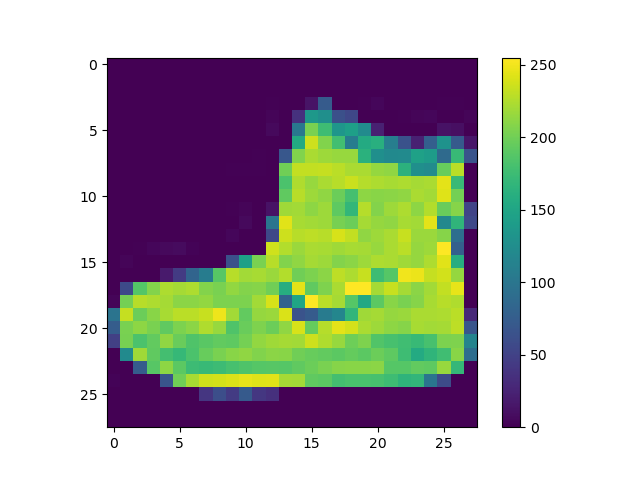
\includegraphics[width=0.8\textwidth]{Images/TensorFlowPackage/preprocessData}
	\caption{Visualization of the pixel values in the first image of the training set.} 
	\label{fig:pixelValues}
\end{figure}

Before training the neural network, data preprocessing is performed by scaling pixel values to a range of 0 to 1 (See Listing \ref{code:dataPreprocessing}). It is crucial to preprocess both the training set and the testing set in a consistent manner.

\begin{code}[h!]
	\lstinputlisting[language=Python, numbers=none, linerange={150-152}]{Code/TensorFlow/clothingimgClassification.py}    
	
	\caption{Data preprocessing to scale pixel values to the range [0, 1].}
	\label{code:dataPreprocessing}
\end{code}

To ensure that the data is appropriately formatted and that you are prepared to construct and train the network, let's showcase the initial 25 images from the training set. Additionally, we'll display the corresponding class names beneath each image (See Listing \ref{code:displayImages} and Figure \ref{fig:first25Images}).

\begin{code}[h!]
	\lstinputlisting[language=Python, numbers=none, linerange={162-171}]{Code/TensorFlow/clothingimgClassification.py}    
	
	\caption{Displaying the initial 25 images from the training set with class names.}
	\label{code:displayImages}
\end{code}

\begin{figure}[h!]
	\centering
	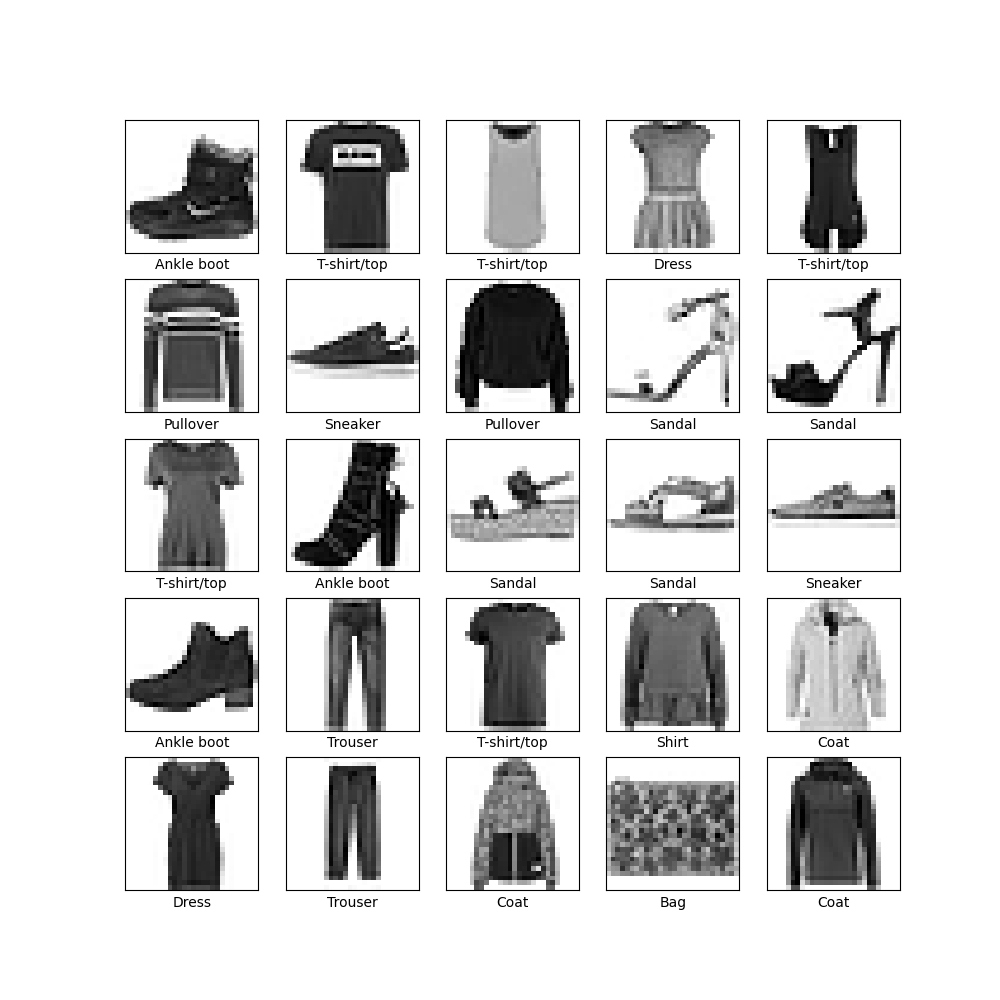
\includegraphics[width=0.8\textwidth]{Images/TensorFlowPackage/first25TrainingImages}
	\caption{Visualization of the initial 25 images from the training set with corresponding class names.} 
	\label{fig:first25Images}
\end{figure}

\subsection{Building the Model}

Creating a neural network involves configuring its layers and subsequently compiling the model. Layers are responsible for extracting representations from the input data, with the expectation that these representations prove insightful for addressing the given problem.

The majority of deep learning involves connecting basic layers in a sequence. Many layers, such as \PYTHON{tf.keras.layers.Dense}, possess parameters that are fine-tuned during the training process (See Listing \ref{code:modelLayers}).

\begin{code}[h!]
	\lstinputlisting[language=Python, numbers=none, linerange={182-186}]{Code/TensorFlow/clothingimgClassification.py}    
	
	\caption{Defining the layers of the neural network model.}
	\label{code:modelLayers}
\end{code}

The initial layer in this network, \PYTHON{tf.keras.layers.Flatten}, transforms the format of the images from a two-dimensional array (28 by 28 pixels) to a one-dimensional array (28 $\times$ 28 = 784 pixels). Visualize this layer as the process of unstacking rows of pixels in the image and aligning them in a linear fashion. This layer does not involve learning any parameters; its sole function is to reformat the data.

Following the flattening process, the network comprises a series of two \PYTHON{tf.keras.layers.Dense} layers. These layers are densely connected, or fully connected, neural layers. The initial \PYTHON{Dense} layer consists of 128 nodes (or neurons), while the subsequent (and final) layer produces a logits array with a length of 10. Each node holds a score indicating the likelihood that the current image belongs to one of the 10 classes.


\subsubsection{Compiling the Model}

Prior to initiating the model training, a few additional configurations are necessary (See Listing \ref{code:modelCompilation}). These adjustments are incorporated during the model's compilation phase:

\begin{itemize}
	\item \textbf{Optimizer:} This determines how the model is updated based on the observed data and its associated loss function.
	
	\item \textbf{Loss function:} This metric gauges the accuracy of the model during training, with the objective of minimizing the function to guide the model in the correct direction.
	
	\item \textbf{Metrics:} These are employed to monitor both the training and testing phases. In the present example, accuracy is utilized as a metric, representing the fraction of images that are accurately classified.
\end{itemize}

\begin{code}[h!]
	\lstinputlisting[language=Python, numbers=none, linerange={204-206}]{Code/TensorFlow/clothingimgClassification.py}    
	
	\caption{Compiling the neural network model with optimizer, loss function, and metrics.}
	\label{code:modelCompilation}
\end{code}


\subsection{Training the Model}

Training the neural network model involves the following steps:

\begin{enumerate}
	\item Feed the training data into the model. In this instance, the training data is stored in the \PYTHON{trainImages} and \PYTHON{trainLabels} arrays.
	
	\item The model learns to establish associations between images and labels.
	
	\item Utilize the trained model to make predictions on a test set—here, represented by the \PYTHON{testcimages} array.
	
	\item Verify the accuracy of predictions by comparing them to the labels in the \PYTHON{testLabels} array.
\end{enumerate}

To train the neural network model see Listing \ref{code:modelTraining}.

\begin{code}[h!]
	\lstinputlisting[language=Python, numbers=none, linerange={211}]{Code/TensorFlow/clothingimgClassification.py}    
	
	\caption{Training the neural network model}
	\label{code:modelTraining}
\end{code}

\begin{verbatim}
	...
	Epoch 9/10
	1875/1875 [==============================] - 4s 2ms/step - loss: 0.2481 - accuracy: 0.9072
	Epoch 10/10
	1875/1875 [==============================] - 4s 2ms/step - loss: 0.2392 - accuracy: 0.9102
\end{verbatim}

Throughout the training process, the metrics of loss and accuracy are presented. This particular model attains an accuracy of approximately 91\% on the training data. Note that without the normalizing step in Listing \ref{code:dataPreprocessing}, the accuracy was about 80\%. This shows the effect of this step in the process.

A loss of 0.2392 represents the average loss on the training dataset for the current epoch. The loss is a measure of how well the model is performing, with lower values indicating better performance.


\subsubsection{Evaluation}

Evaluate the model's performance on the test dataset in Listing \ref{code:modelEvaluation}:

\begin{code}[h!]
	\lstinputlisting[language=Python, numbers=none, linerange={224-226}]{Code/TensorFlow/clothingimgClassification.py}    
	
	\caption{Evaluating the neural network model on the test dataset.}
	\label{code:modelEvaluation}
\end{code}

\begin{verbatim}
	313/313 - 1s - loss: 0.3383 - accuracy: 0.8817 - 556ms/epoch - 2ms/step
	
	Test accuracy: 0.8816999793052673
\end{verbatim}

It turns out that the accuracy on the test dataset is a little less than the accuracy on the training dataset. This gap between training accuracy and test accuracy represents overfitting. Overfitting happens when a machine learning model performs worse on new, previously unseen inputs than it does on the training data. An overfitted model "memorizes" the noise and details in the training dataset to a point where it negatively impacts the performance of the model on the new data.

\subsection{Making Predictions}

Having trained the model, you can employ it to generate predictions for certain images (See Listing \ref{code:makePredictions}). Append a softmax layer to transform the model's linear outputs—logits—into probabilities, facilitating a more intuitive interpretation.

\begin{code}[h!]
	\lstinputlisting[language=Python, numbers=none, linerange={239-240}]{Code/TensorFlow/clothingimgClassification.py}    
	
	\caption{Making predictions using the trained neural network model}
	\label{code:makePredictions}
\end{code}

\begin{verbatim}
	313/313 [==============================] - 0s 1ms/step
\end{verbatim}

The model has provided predictions for the label of each image in the testing set. Let's examine the first prediction in Listing \ref{code:predictionArray}:

\begin{code}[h!]
	\lstinputlisting[language=Python, numbers=none, linerange={242}]{Code/TensorFlow/clothingimgClassification.py}    
	
	\caption{producing the prediction array for the first image in the testing set}
	\label{code:predictionArray}
\end{code}

{\footnotesize
	\begin{verbatim}
		[1.6619989e-08 1.4881327e-09 8.5905718e-09 4.6579121e-08 7.5430655e-08
		6.0041228e-05 2.0011402e-07 2.5325418e-03 6.7323890e-07 9.9740642e-01]
	\end{verbatim}
}

A prediction comprises an array of 10 numbers, indicating the model's "confidence" in associating the image with each of the 10 distinct articles of clothing. Identify the label with the highest confidence value:

Hence, the model expresses the highest confidence in categorizing this image as an ankle boot, corresponding to the \PYTHON{classNames[9]}. Verifying the test label confirms the accuracy of this classification (See Listing \ref{code:verifyLabels}):

\begin{code}[h!]
	\lstinputlisting[language=Python, numbers=none, linerange={243-244}]{Code/TensorFlow/clothingimgClassification.py}    
	
	\caption{Verifying the predicted and actual labels for the image.}
	\label{code:verifyLabels}
\end{code}


\begin{verbatim}
	9
	9
\end{verbatim}

\subsection{Verify Predictions}

After training the model, you can utilize it to make predictions on specific images (See Listings \ref{code:predictionPlotZero} and \ref{code:PredictionsZeroTwelve} and Figures \ref{fig:predictionPlotZero} and \ref{fig:PredictionsZeroTwelve}). Let's examine the predictions for the 0th and 12th images, showcasing correct predictions in blue and incorrect predictions in red.

\begin{code}[h!]
	\lstinputlisting[language=Python, numbers=none, linerange={311-318}]{Code/TensorFlow/clothingimgClassification.py}    
	
	\caption{Code for visualizing predictions on the 0th image}
	\label{code:predictionPlotZero}
\end{code}

\begin{figure}[h!]
	\centering
	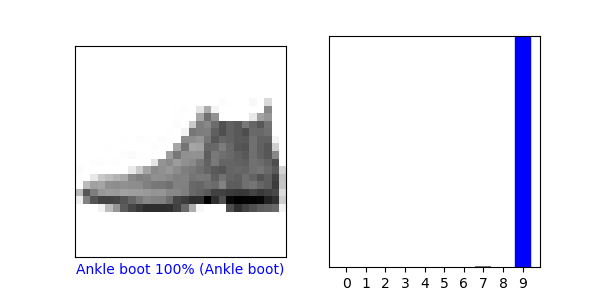
\includegraphics[width=0.8\textwidth]{Images/TensorFlowPackage/predictionPlotZero}
	\caption{Predictions for the 0th image. Correct prediction is in blue.} \label{fig:predictionPlotZero}
\end{figure}

\begin{code}[h!]
	\lstinputlisting[language=Python, numbers=none, linerange={320-327}]{Code/TensorFlow/clothingimgClassification.py}    
	
	\caption{Code for visualizing predictions on the 12th image}
	\label{code:PredictionsZeroTwelve}
\end{code}

\begin{figure}[h!]
	\centering
	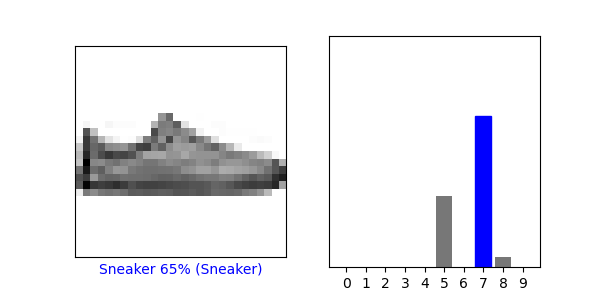
\includegraphics[width=0.8\textwidth]{Images/TensorFlowPackage/predictionPlotTwelve}
	\caption{Predictions for the 12th image. Correct prediction is in blue} \label{fig:PredictionsZeroTwelve}
\end{figure}

Visualize multiple images along with their corresponding predictions is shown in Listing \ref{code:predictionPlots}. The result is shown in \ref{fig:predictionPlots}.It's important to acknowledge that the model may make errors despite exhibiting high confidence.

\begin{code}[h!]
	\lstinputlisting[language=Python, numbers=none, linerange={340-351}]{Code/TensorFlow/clothingimgClassification.py}    
	
	\caption{Code for visualizing predictions for multiple images}
	\label{code:predictionPlots}
\end{code}

\begin{figure}[h!]
	\centering
	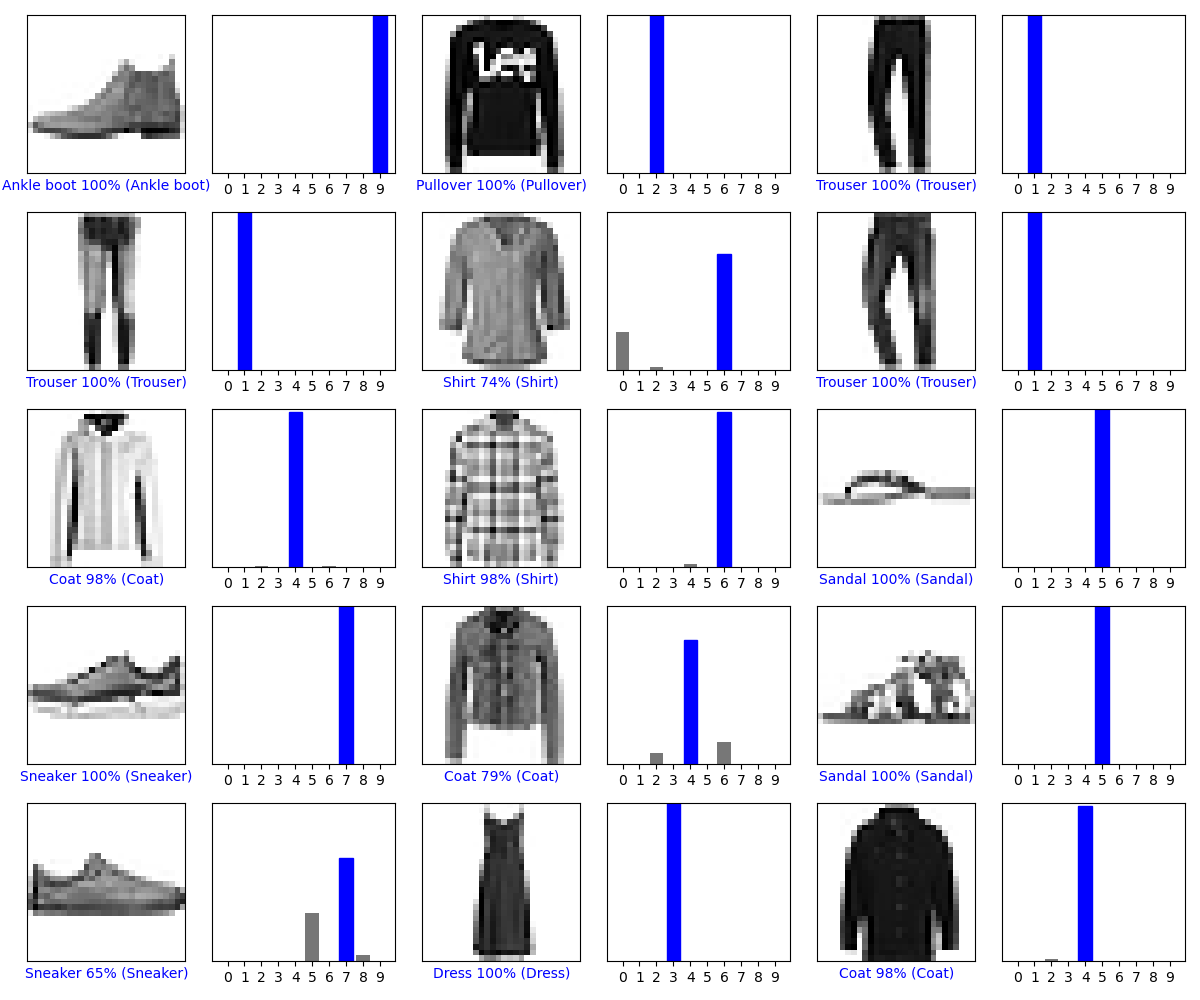
\includegraphics[width=0.8\textwidth]{Images/TensorFlowPackage/predictionPlots}
	\caption{Visualizing predictions for multiple images} \label{fig:predictionPlots}
\end{figure}

\subsection{Use the Trained Model}

Finally, leverage the trained model to predict a single image (See Listing \ref{code:predictSingleImage}).

\begin{code}[h!]
	\lstinputlisting[language=Python, numbers=none, linerange={358-360}]{Code/TensorFlow/clothingimgClassification.py}    
	
	\caption{Code for predicting a single image}
	\label{code:predictSingleImage}
\end{code}

\begin{verbatim}
	(28, 28)
\end{verbatim}

Optimized for batch processing, tf.keras models excel at making predictions on collections of examples simultaneously. Therefore, even when working with a single image, it is necessary to include it in a list (See Listing \ref{code:prepareSingleImage}).

\begin{code}[h!]
	\lstinputlisting[language=Python, numbers=none, linerange={363-364}]{Code/TensorFlow/clothingimgClassification.py}    
	
	\caption{Preparing a single image for prediction by adding it to a list.}
	\label{code:prepareSingleImage}
\end{code}

\begin{verbatim}
	(1, 28, 28)
\end{verbatim}

Predicting the accurate label for this image is shown in \ref{code:makeDinglePrediction}.

\begin{code}[h!]
	\lstinputlisting[language=Python, numbers=none, linerange={368-369}]{Code/TensorFlow/clothingimgClassification.py}    
	
	\caption{Making predictions for a single image.}
	\label{code:makeDinglePrediction}
\end{code}

{\footnotesize
	\begin{verbatim}
		1/1 [==============================] - 0s 23ms/step
		[[8.4762414e-06 2.3953922e-11 9.9964368e-01 1.5056546e-11 3.0798238e-04
		8.6492816e-16 3.9860388e-05 3.5954907e-23 6.0896788e-11 4.6433261e-12]]
	\end{verbatim}
}

To display the predicted probabilities for each class see Listing \ref{code:displayProbabilities} and Figure \ref{fig:singlePredictionPlot}.

\begin{code}[h!]
	\lstinputlisting[language=Python, numbers=none, linerange={371-374}]{Code/TensorFlow/clothingimgClassification.py}    
	
	\caption{Displaying the predicted probabilities for each class.}
	\label{code:displayProbabilities}
\end{code}

\begin{figure}[h!]
	\centering
	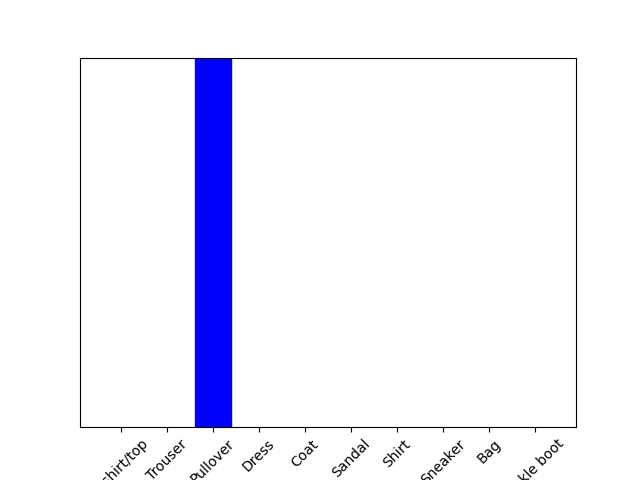
\includegraphics[width=0.8\textwidth]{Images/TensorFlowPackage/singlePredictionPlot}
	\caption{Prediction for a single image} \label{fig:singlePredictionPlot}
\end{figure}

See Listing \ref{code:extractPredictions} to extract the predictions for the sole image in the batch:

\begin{code}[h!]
	\lstinputlisting[language=Python, numbers=none, linerange={376}]{Code/TensorFlow/clothingimgClassification.py}    
	
	\caption{Extracting predictions for the sole image in the batch}
	\label{code:extractPredictions}
\end{code}

\begin{verbatim}
	(1, 28, 28)
\end{verbatim}

\subsection{Saving the Model}

A TensorFlow model is saved in the SavedModel format using the \PYTHON{model.save()} method, with the saved path specified as \PYTHON{"./savedModel"} (See Listing \ref{code:saveandConvertModel}). Following this, the SavedModel is converted to the TensorFlow Lite format using \PYTHON{tf.lite.TFLiteConverter.from\_saved\_model()}. The resulting TensorFlow Lite model is then saved to a file, and the path for the TensorFlow Lite model is set as \PYTHON{"./savedModel/model.tflite"}. This process is essential for deploying the model in resource-constrained environments, such as mobile or edge devices, where the lightweight TensorFlow Lite format enhances efficient model inference.

\begin{code}[h!]
	\lstinputlisting[language=Python, numbers=none, linerange={391-402}]{Code/TensorFlow/clothingimgClassification.py}    
	
	\caption{Saving the TensorFlow model in the SavedModel format and converting it to TensorFlow Lite}
	\label{code:saveandConvertModel}
\end{code}


\section{Further Readings}

\begin{itemize}
	\item The article "Deep Learning With TensorFlow: A Review" \cite{Pang:2020} explores the core concepts of TensorFlow, a leading deep learning library initially developed by Google. It highlights TensorFlow's widespread popularity and applications, particularly in educational and behavioral sciences. The review covers key neural network models and optimization methods, emphasizing TensorFlow's role in simplifying implementation challenges. Essential TensorFlow features, such as graph construction functions and TensorBoard visualization, are discussed, with a practical application example of training a convolutional neural network for handwritten digit classification. The article concludes by comparing low- and high-level APIs, touching on GPU support, distributed training, and the TensorFlow Probability library for probabilistic modeling.
	\item "Hands-On Machine Learning with Scikit-Learn, Keras, and TensorFlow" \cite{Geron:2022} is an accessible guide for beginners in machine learning. The book aims to provide readers with the concepts and tools needed to implement programs that learn from data. Scikit-Learn is introduced for its simplicity and efficiency, while TensorFlow is explored for distributed numerical computation, particularly in training large neural networks. The high-level deep learning API, Keras, integrated with TensorFlow, simplifies the training and execution of neural networks. With a hands-on approach, the book emphasizes practical examples and minimal theory to foster an intuitive understanding of machine learning concepts.
	\item The article "A Tour of TensorFlow" \cite{Goldsborough:2016} provides a thorough review of TensorFlow. The paper contextualizes TensorFlow within the realm of modern deep learning concepts and software, covering its computational paradigms, distributed execution model, programming interface, and visualization tools. Goldsborough conducts a qualitative and quantitative comparison with alternative libraries, discussing the rise of deep learning in recent years. The review concludes by exploring real-world use-cases of TensorFlow in academia and industry, offering a comprehensive overview of its contributions to machine learning.
	\item The book "Introduction to TensorFlow 2.0" \cite{Singh:2019} is a practical guide that delves into the key changes made by Google's TensorFlow team. The book covers data processing, building machine learning models, including neuro-linguistic programming, and deploying models in production. Aimed at data analysts, engineers, and newcomers to data science and machine learning, the book stands out for its simplicity, real-world applications, and inclusion of case studies. Overall, it provides valuable insights into TensorFlow 2.0's fundamentals and practical use.
\end{itemize}









